\documentclass[a4paper,11pt]{article}
\usepackage{a4wide}
\usepackage{graphicx}

\title{eXamine: Exploring annotated modules in networks\\Supplemental Text}

\author{K.~Dinkla, M.~El-Kebir, C-I.~Bucur\\M.~Siderius, M.J.~Smit, G.W.~Klau,
M.A.~Westenberg}

%\date{}

\begin{document}
\maketitle
\tableofcontents

\section{Introduction}
This case study demonstrates how to use eXamine to study an annotated module
in Cytoscape. The module that we study has 17 nodes and 18 edges and occurs
within the KEGG mouse network consisting of 3863 nodes and 29293 edges. The
module is annotated with sets from four different categories: (1) KEGG pathways
and the GO categories (2) molecular process, (3) biological function and (4)
cellular component. To perform this use case, you need to download the following
three files. 
\begin{enumerate}
  \item \texttt{edges.txt}: contains the edges of the KEGG mouse network.
    \begin{verbatim}
    URL: https://github.com/melkebir/examine/blob/master/data/edges.txt
    \end{verbatim}
  \item \texttt{nodes\_induced.txt}: contains additional node annotation and
    set membership information for nodes that are part of the module.
    \begin{verbatim}
    URL: https://github.com/melkebir/examine/blob/master/data/nodes_induced.txt
    \end{verbatim}
  \item \texttt{sets\_induced.txt}: contains additional information on the sets
    such as a URL, a small description and an enrichment $p$-value.
    \begin{verbatim}
    URL: https://github.com/melkebir/examine/blob/master/data/sets_induced.txt
    \end{verbatim}
\end{enumerate}

\section{Use case}

\subsection{Importing edges and node annotation}

In the following we give instructions for importing the edges and the node based
annotation. Note that it is important to ensure that set-membership
information is imported as `List of String' type.

\begin{enumerate}
  \item Start Cytoscape and close the Welcome screen.
  \item Import the network defined in \texttt{edges.txt} via File $\rightarrow$
    Import $\rightarrow$ Network $\rightarrow$ File\ldots
  \begin{enumerate}
    \item Set `Source Interaction' to `Column 1' and `Target Interaction' to
      `Column 2'.
      \begin{center}
        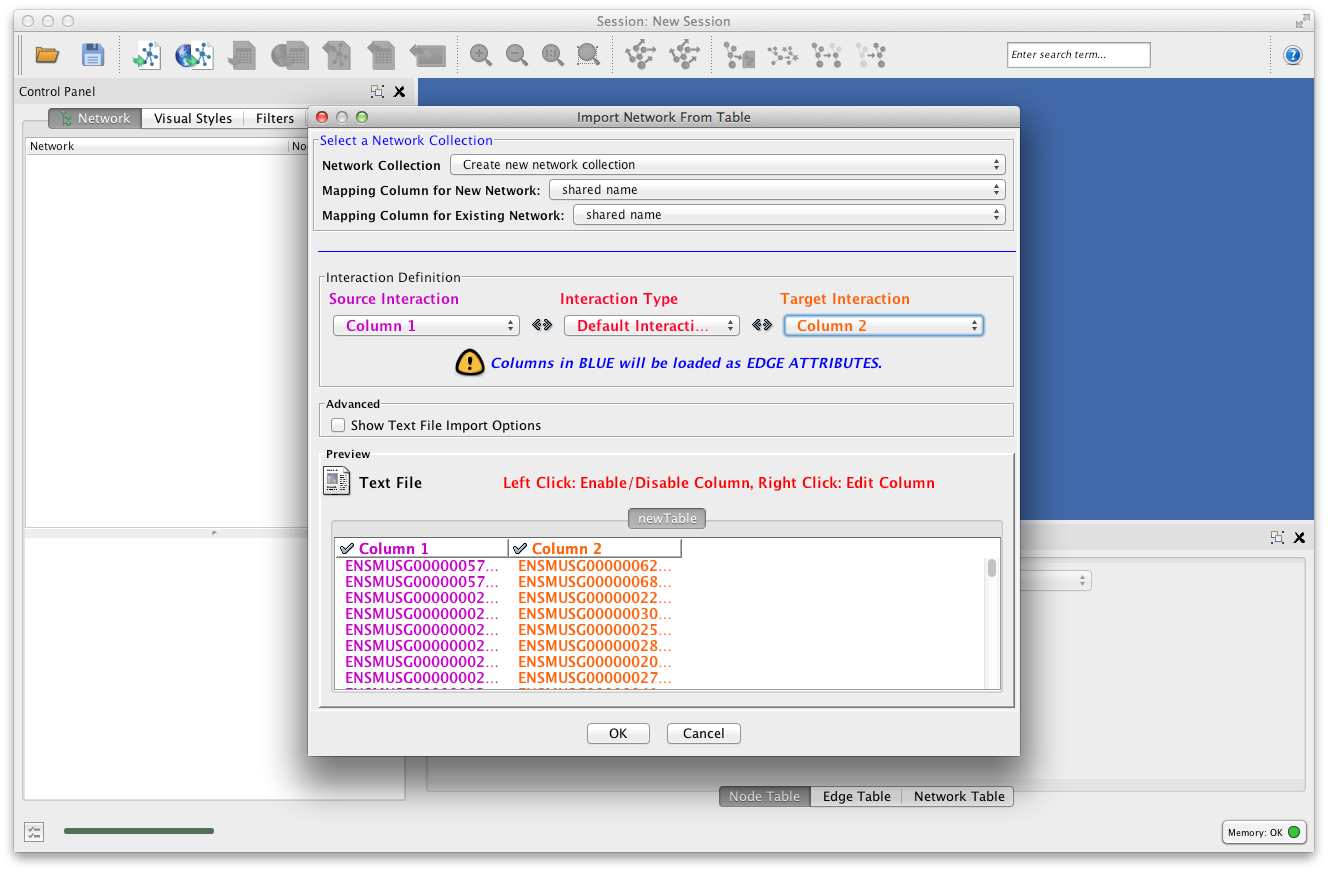
\includegraphics[width=.9\textwidth]{images/1.png}
      \end{center}
    \end{enumerate}
  \item Import node annotation in \texttt{nodes\_induced.txt} via File
    $\rightarrow$ Import $\rightarrow$ Table $\rightarrow$ File\ldots
    \begin{enumerate}
      \item Click on `Show Text File Import Options'.
      \item Click on `Transfer first line as column names'.
      \item Scroll all the way to the right in the table, so that the columns
        Process, Function, Component and Pathway are visible.
      \item Now right click on the column header `Process'.
      \item Set the column type to `List of Strings' with `$|$' as the delimiter
        and press OK.
      \item Repeat (d) and (e) for columns Function, Component and Pathway.
      \item Press OK.
        \begin{center}
          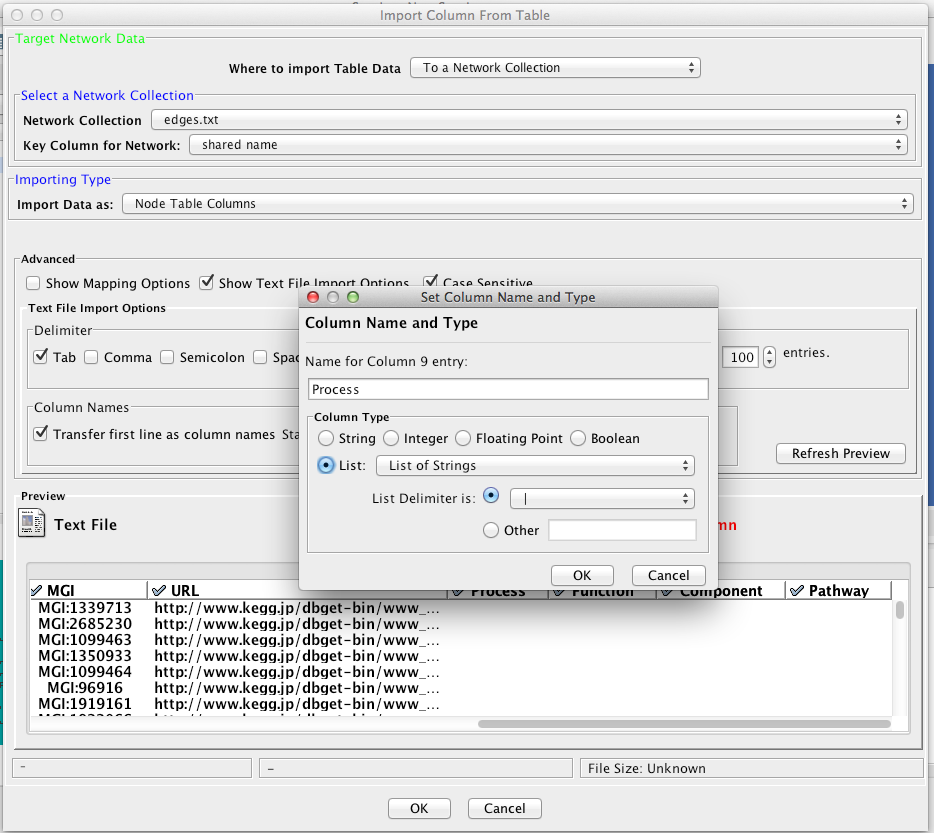
\includegraphics[width=.7\textwidth]{images/2.png}
        \end{center}
    \end{enumerate}
\end{enumerate}

\subsection{Importing set annotation}

In this subsection we describe how to import the set based annotations. In order
to do so, eXamine needs to generate group nodes for each of the sets present in the
module. Before doing so we need to select nodes present in the module; these
nodes have the value `small' in column `Module'. We do this using Cytoscape's
filter functionality.

\begin{enumerate}
  \item Go to the `Filters' pane in the `Control panel'.
  \item Select the column `node.Module' and press `Add'.
  \item Select `small' in the combo box.
  \item Press `Apply Filter'.
  \item Now remove the filter by clicking on the recycle bin.
  \begin{center}
    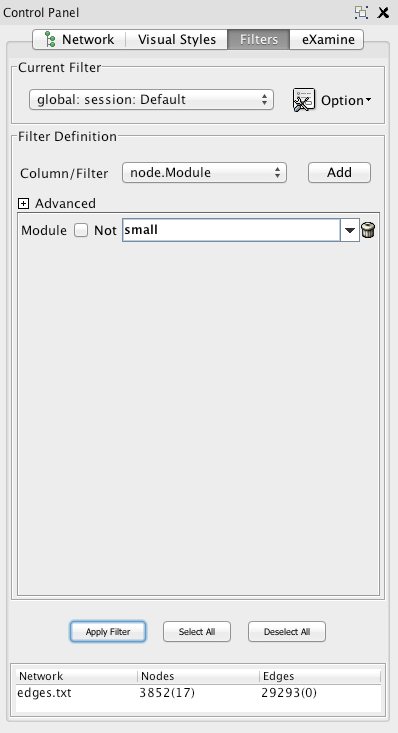
\includegraphics[width=.4\textwidth]{images/3.png}
    \hspace{1cm}
    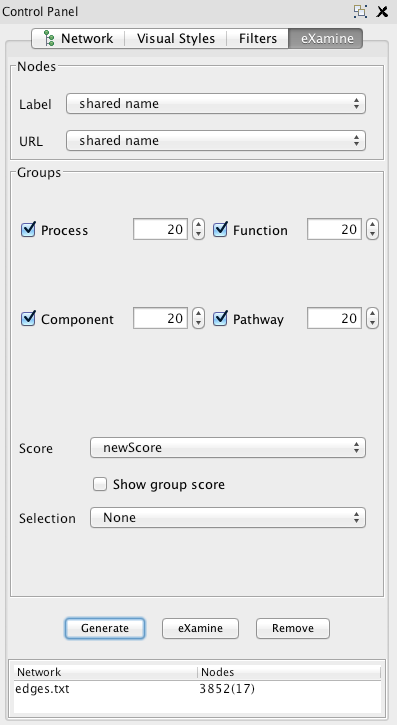
\includegraphics[width=.4\textwidth]{images/4.png}
  \end{center}
\end{enumerate}

Now that we have selected the nodes of the module, we can proceed to generating
group nodes for each set.

\begin{enumerate}
  \setcounter{enumi}{5}
  \item Go to the `eXamine' pane in the `Control panel'.
  \item Select all four categories `Process', `Function', `Component' and `Pathway'.
  \item Press `Generate'.
  \item Wait until the task `Generate groups' is done (should take just a few
    seconds).
\end{enumerate}

The next step is to import the set-based annotation.

\begin{enumerate}
  \setcounter{enumi}{9}
  \item Import node annotation in \texttt{sets\_induced.txt} via File
    $\rightarrow$ Import $\rightarrow$ Table $\rightarrow$ File\ldots
    \begin{enumerate}
      \item Click on `Show Text File Import Options'.
      \item Click on `Transfer first line as column names'.
      \item Press OK.
    \end{enumerate}
\end{enumerate}

\subsection{Starting and using eXamine}

Next we describe how to start eXamine. Before doing so, make sure that the 17
nodes of the module are selected. If they are not, go to the previous sub
section for instructions on how to select them.

\begin{enumerate}
  \item Go to the `eXamine' pane in the `Control panel'.
  \item Set `Label' to `Symbol'.
  \item Set `URL' to `URL'.
  \item Select all four categories `Process', `Function', `Component' and `Pathway'.
  \item Set `Score' to `Score'.
  \item Click on `Show group score'.
  \item Press `eXamine' and maximize the new window that pops up.
  \begin{center}
    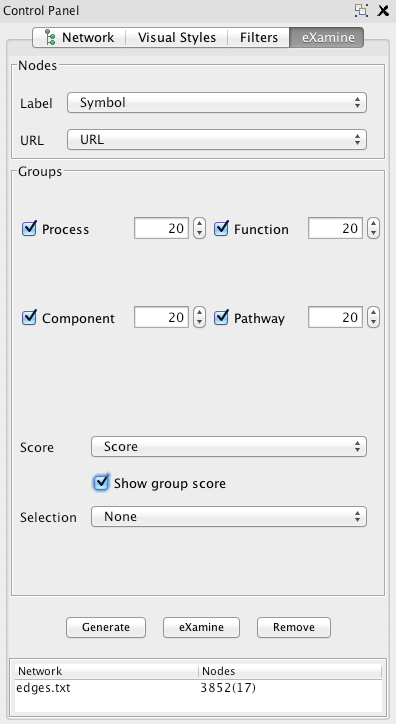
\includegraphics[width=.4\textwidth]{images/5.png}
  \end{center}
\end{enumerate}

In the eXamine window sets can be made active and additional information can be
requested.

\begin{enumerate}
  \setcounter{enumi}{7}
  \item Select the GO terms `beta-catenin binding', `growth factor
    activity', and KEGG pathways `Phosphatidylinositol signaling', `Pathways in
    cancer', and `Adherens junction'.
    \begin{center}
      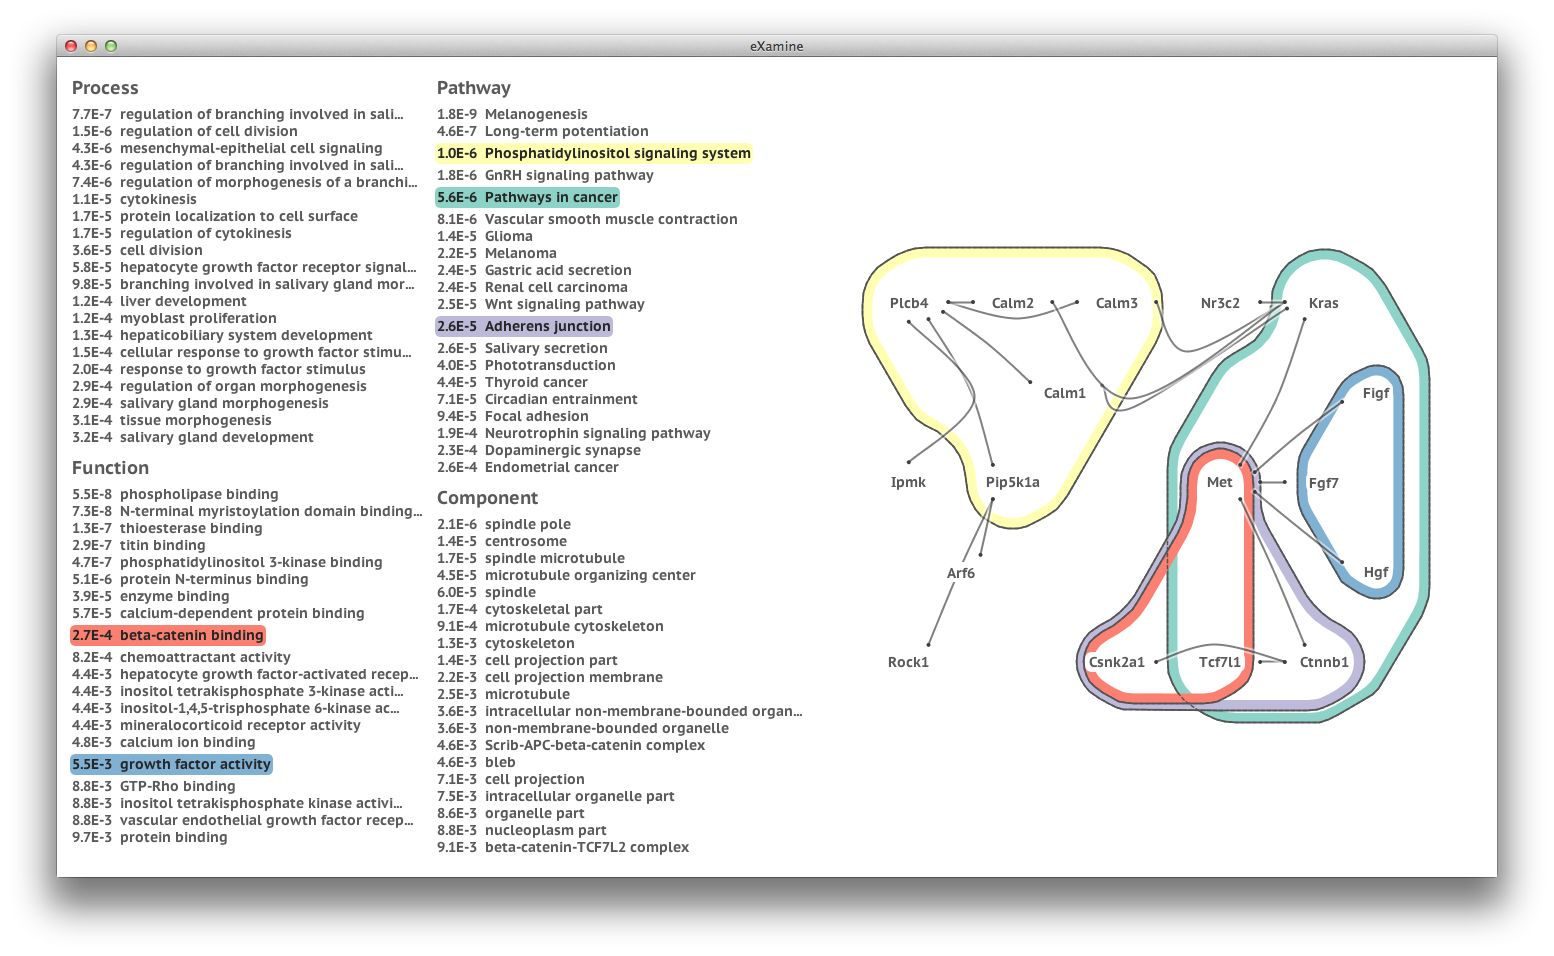
\includegraphics[width=\textwidth]{images/6.png}
    \end{center}
  \item To adjust the set dominance of one the selected sets hover over either
    the set label or the corresponding contour and spin the mouse wheel.
  \item Additional node information can be requested by Ctrl-clicking on a node.
  \item Similarly Ctrl-clicking on a set gives additional information about that
    set.
\end{enumerate}

To color the labels we need to set the node fill color.

\begin{enumerate}
  \setcounter{enumi}{11}
  \item Go to the `Visual Styles' pane in the `Control panel'.
  \item Click on `Fill Color'.
  \item Set `Column' to `newScore' and `Mapping Type' to `Continuous Mapping'.
  \item Double click on the color map.
  \item Set the dialog box as follows.
    \begin{center}
      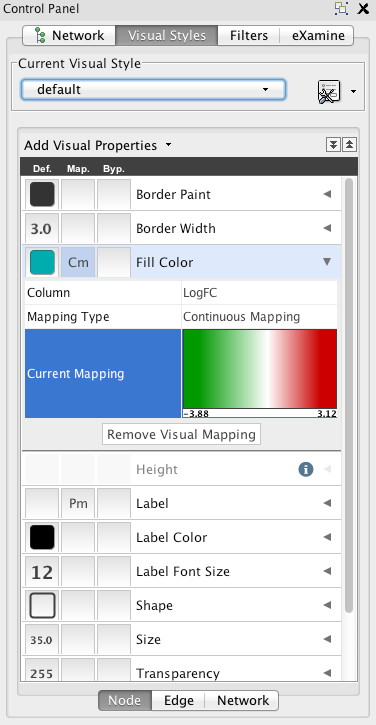
\includegraphics[width=.4\textwidth]{images/7.png}
      \hspace{1cm}
      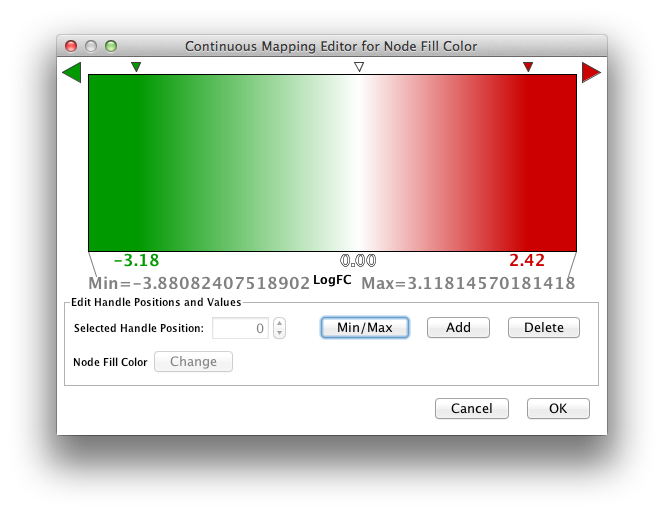
\includegraphics[width=.4\textwidth]{images/8.png}
    \end{center}
  \item Now the module looks as follows.
    \begin{center}
      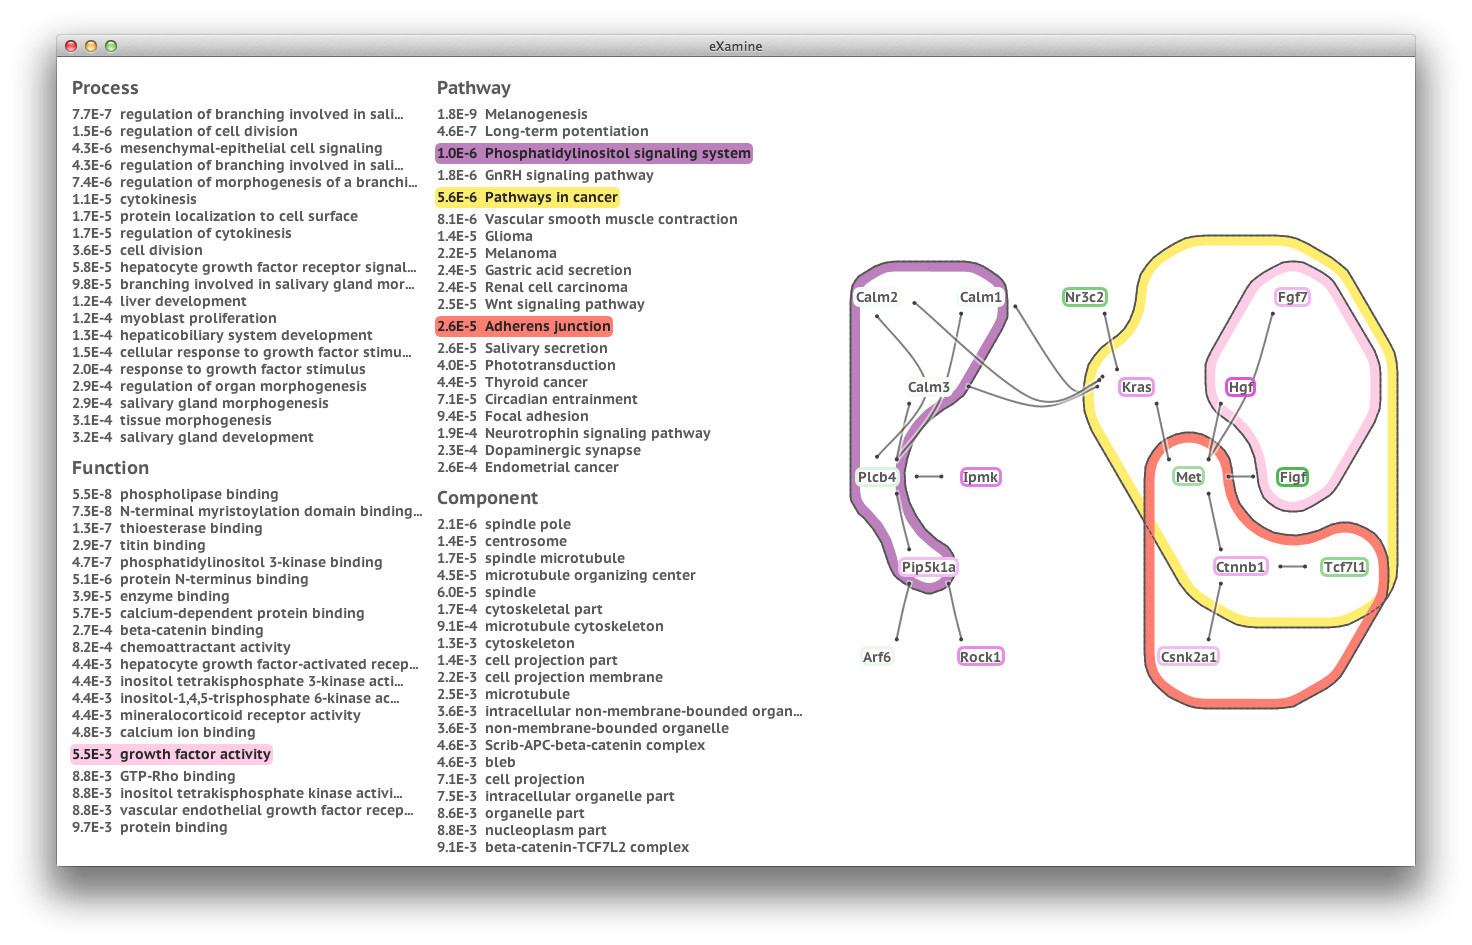
\includegraphics[width=.9\textwidth]{images/9.png}
    \end{center}
\end{enumerate}

\end{document}
